\section{Matrix-free modal identification of a fluid-loaded plate}\label{sec:vf-fsi}

\subsection*{Concept and purpose}

\citet{liu2026fsi} identify the natural frequencies, damping ratios and mode shapes of a fluid-loaded structure from scalar frequency-response samples at one reference point, without access to the mass, damping or stiffness matrices and without knowing the force. A Loewner pencil built from two interleaved sets of sampled frequencies turns the identification into a small generalised eigenproblem, and a screening step that compares many such models separates physical modes from spurious ones. The study tests the method on a steel plate in air and in water: the identification error against a reference, the effect of mesh, boundary condition, excitation, sample density, band, sensor position and noise, and the quality of the recovered mode shapes. It is the study that uses \rom{}'s Loewner and screening modules (\anchor{rom_engine.loewner}, \anchor{rom_engine.screening}) on a model from \fea{}.

\subsection*{Mathematics as implemented}

A linear structure, possibly fluid-loaded, responds to a harmonic force $\mathbf Fe^{i\omega t}$ with
\begin{equation}\label{eq:fsi-frf}
\mathbf x(\omega)=\mathbf T(\omega)^{-1}\mathbf F,\qquad\mathbf T(\omega)=\mathbf K+i\omega\mathbf C-\omega^2\mathbf M\quad(-\,\omega^2\mathbf M_f(\omega)\ \text{if fluid-loaded}).
\end{equation}
The modal parameters are the complex roots $\omega_k^\ast$ of $\det\mathbf T(\omega)=0$, reported as $f_k=\operatorname{Re}\omega_k^\ast/2\pi$ and $\eta_k=\operatorname{Im}\omega_k^\ast/\operatorname{Re}\omega_k^\ast$.

\emph{Loewner pencil.} Two disjoint interpolation sets $\{\omega_a\}_{a=1}^n$ and $\{\omega_b\}_{b=1}^n$ give samples $x_a=x(\omega_a)$, $x_b=x(\omega_b)$ and the $n\times n$ matrices
\begin{equation}\label{eq:fsi-loewner}
\tilde A_{ab}=\frac{\omega_a^{2}x_a-\omega_b^{2}x_b}{\omega_a^{2}-\omega_b^{2}},\qquad
\tilde E_{ab}=\frac{x_a-x_b}{\omega_a^{2}-\omega_b^{2}},\qquad
\tilde A\tilde\Phi=\tilde E\tilde\Phi\tilde\Lambda,\quad\lambda_i=\omega_i^2 .
\end{equation}
For a frequency-independent system each response is a rational function of $\lambda=\omega^2$, $x(\lambda)=N(\lambda)/D(\lambda)$ with $\deg D$ equal to the number of modes; the divided differences are its Loewner matrices and the generalised eigenvalues are its poles, the complex squared natural frequencies with damping included. With exact data and $n$ at least the number of modes in the data, the poles are recovered to round-off; a larger $n$ produces extra, non-physical eigenpairs that the screening removes.

\emph{Mode shapes.} Responses at $m$ measurement points sampled at the same $\{\omega_b\}$, $\mathbf X_\beta\in\mathbb C^{m\times n}$, give $\boldsymbol\Phi=\mathbf X_\beta\tilde\Phi$, compared with reference shapes by the modal assurance criterion
\begin{equation}\label{eq:fsi-mac}
\mathrm{MAC}(\boldsymbol\phi_a,\boldsymbol\phi_b)=\frac{|\boldsymbol\phi_a^{H}\boldsymbol\phi_b|^{2}}{(\boldsymbol\phi_a^{H}\boldsymbol\phi_a)(\boldsymbol\phi_b^{H}\boldsymbol\phi_b)} .
\end{equation}

\emph{Screening.} (1) $N_{\rm ROM}=25$ Loewner models are built from random disjoint subsets of a pool of sampled frequencies; eigenpairs outside the band or with $\eta\notin[0,1]$ are discarded. (2) Eigenpairs of different models are linked when $|f_i-f_j|/\max(f_i,f_j)<\varepsilon_f=0.5\,\%$ and $|\eta_i-\eta_j|/\max(\eta_i,\eta_j)<\varepsilon_\eta=10\,\%$; clusters are the connected components. (3) For each cluster the stability indices are $S_f=1-\sigma_f/\mu_f$, $S_\eta=1-\sigma_\eta/\mu_\eta$ and $S_{\rm total}=S_fS_\eta$. (4) A cluster is a physical mode if $S_{\rm total}>\tau_s=0.95$ and it occurs in at least $N_{\rm ROM}/2$ distinct models. Physical modes reappear at nearly the same $(f,\eta)$ in every model, spurious ones depend on the interpolation points.

\emph{Truth model: fluid loading.} The reference is built with \fea{}. For a baffled plate with nodal areas $S_i$ and node distances $R_{ij}$, the surface pressure is $p_i=i\omega\rho_f\sum_jg_{ij}(\omega)S_jv_j$ with $g_{ij}=e^{-ikR_{ij}}/(2\pi R_{ij})$, $k=\omega/c_f$, and the exact self term of an equal-area disc of radius $a_i=\sqrt{S_i/\pi}$, $S_ig_{ii}=(1-e^{-ika_i})/(ik)$. With $v=i\omega w$ and nodal force $-Sp$ this gives a complex-symmetric, frequency-dependent fluid mass
\begin{equation}\label{eq:fsi-fluid}
\mathbf M_f(\omega)=n_{\rm sides}\,\rho_f\,\mathbf S\,\mathbf G(\omega)\,\mathbf S,\qquad\mathbf T(\omega)=\mathbf K+i\omega\mathbf C_s-\omega^2\big(\mathbf M_s+\mathbf M_f(\omega)\big),
\end{equation}
whose real part is the (mode-dependent) added mass and whose imaginary part is radiation damping. Reference parameters are the roots of $\mathbf T(\omega^\ast)\mathbf v=\mathbf 0$ found by the Rayleigh-functional Newton iteration $\omega\leftarrow\omega-\mathbf v^{T}\mathbf T(\omega)\mathbf v/\mathbf v^{T}\mathbf T'(\omega)\mathbf v$ started from an undamped wet eigensolution. The identification never sees them; the data fed to it are single-degree-of-freedom FRF samples $x(\omega)=[\mathbf T(\omega)^{-1}\mathbf F]_s$ at the sensor.

\emph{Metrics.} Identified modes are matched one-to-one to reference modes by nearest frequency (2\,\% tolerance for noise tests, 1\,\% otherwise), with $e_f=100|f_{\rm id}-f_{\rm ref}|/f_{\rm ref}$ and $e_\eta=100|\eta_{\rm id}-\eta_{\rm ref}|/\eta_{\rm ref}$; ``non-physical'' counts eigenpairs left unmatched after band and $\eta$ filtering.

\subsection*{Geometry and mesh}

The plate is steel, $455\times379\times3$~mm, simply supported on all four edges (clamped for one study), meshed with Mindlin quadrilaterals (\anchor{fea_engine.elements.Quad4MindlinPlate}, three degrees of freedom per node) in a $16\times16$ grid of 289 nodes and 803 free degrees of freedom. The structural damping is Rayleigh, $\mathbf C_s=\alpha\mathbf M_s+\beta\mathbf K$ with $\alpha=7.362$~s$^{-1}$ and $\beta=1.177\times10^{-5}$~s, applied to the structure only. The fluids are air $(\rho_f,c_f)=(1.21,340)$ and water $(1000,1500)$ in SI units, on one face. \Cref{fig:vf-fsi-geom} shows the plate, the nodes of the publication's Table~1 (excitation at node 193, reference sensor at node 50), the mesh with its 64 constrained edge nodes and 225 wetted nodes, the coupling of one node and the three meshes of the mesh study; \Cref{fig:vf-fsi-fluid} shows how strongly the fluid loading depends on frequency and mode.

\begin{figure}[tbp]
\centering
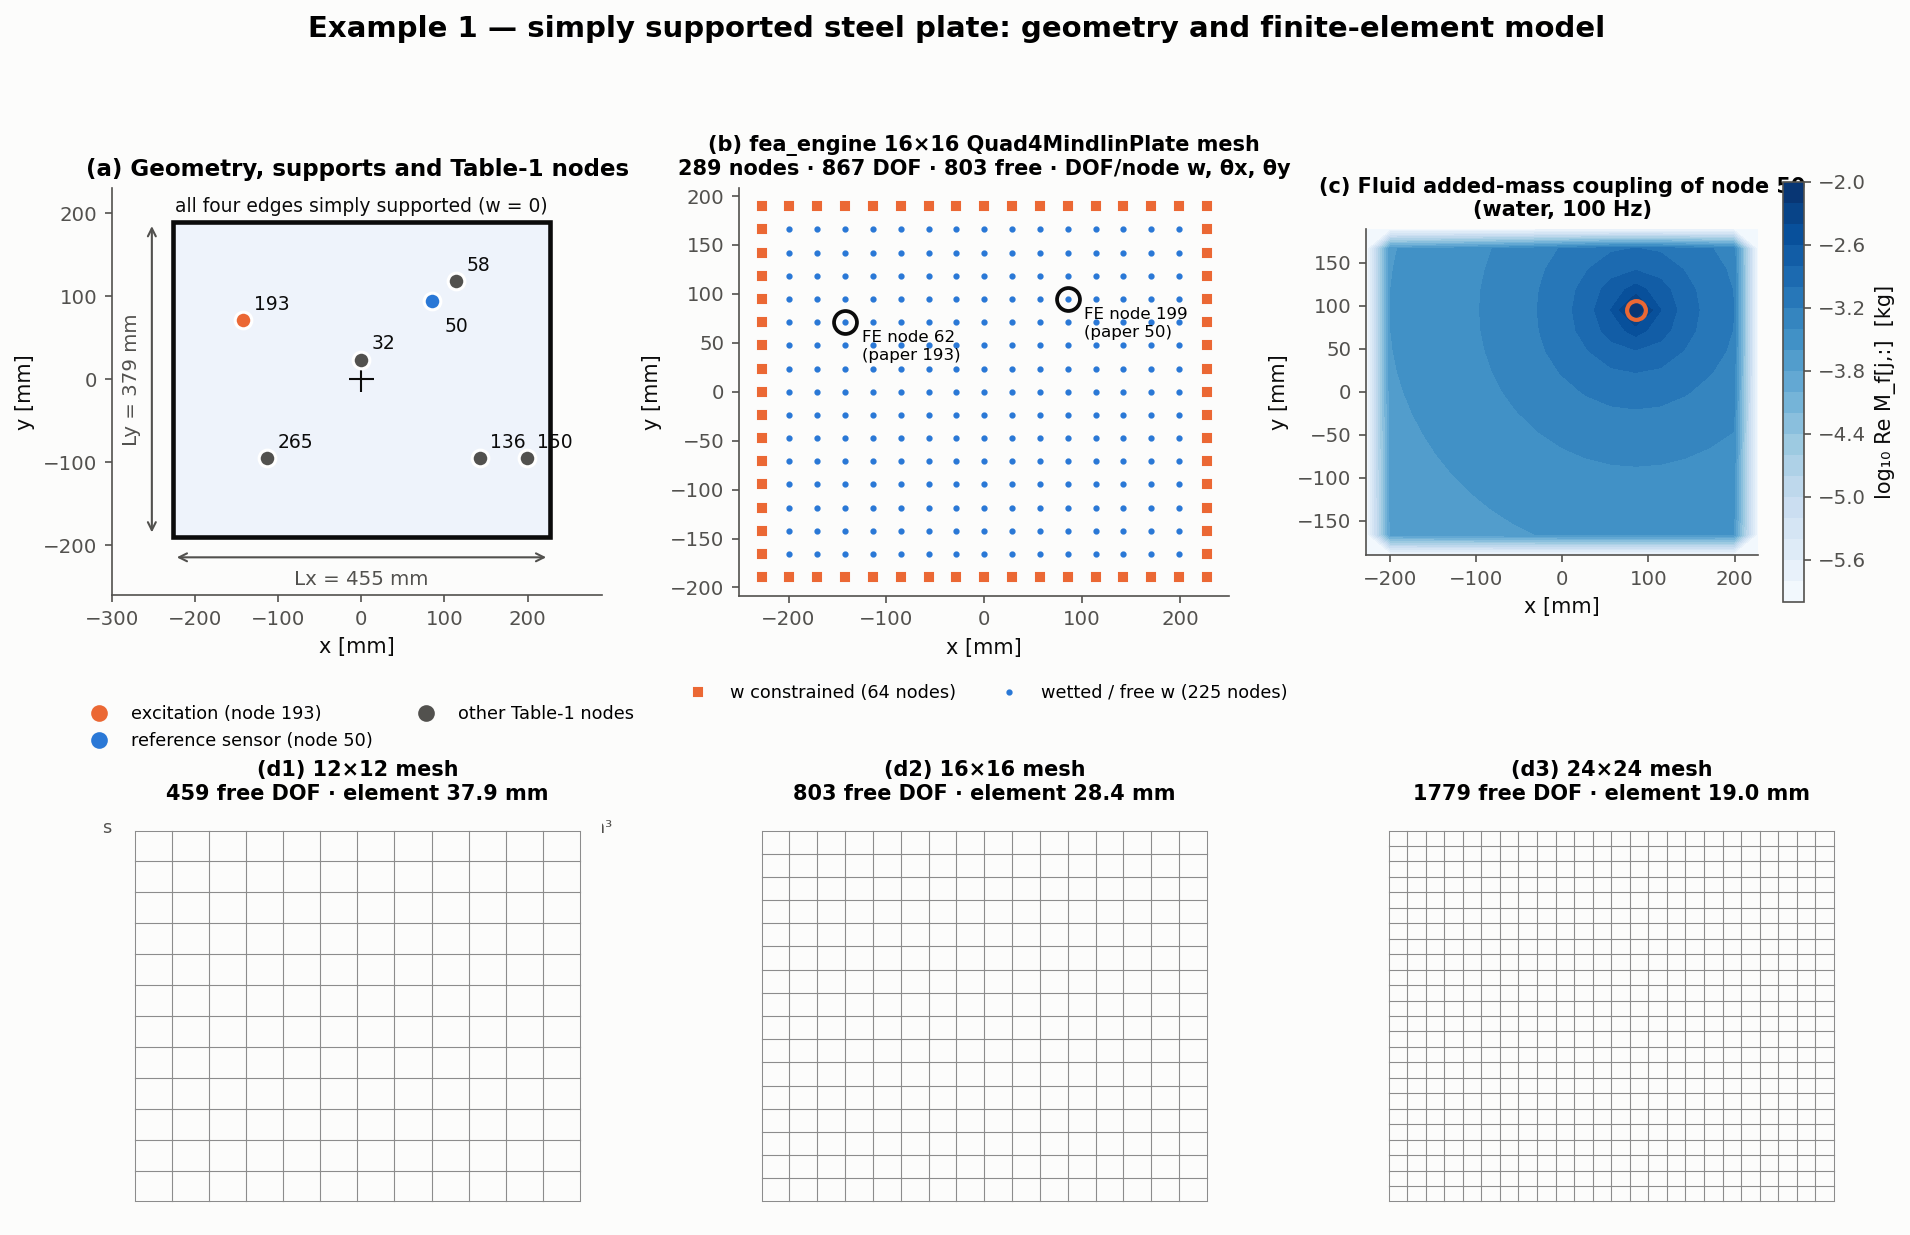
\includegraphics[width=0.98\linewidth]{figures/ch14r/fsi_geom.png}
\caption{Truth model of the identification study. (a) Plate, supports and the nodes of the publication's Table~1. (b) $16\times16$ Mindlin mesh with 64 constrained and 225 wetted nodes. (c) Real part of one row of the fluid added-mass matrix for water at 100~Hz; the coupling decays with distance from the source node. (d) The $12\times12$, $16\times16$ and $24\times24$ meshes of the mesh study.}\label{fig:vf-fsi-geom}
\end{figure}

\begin{figure}[tbp]
\centering
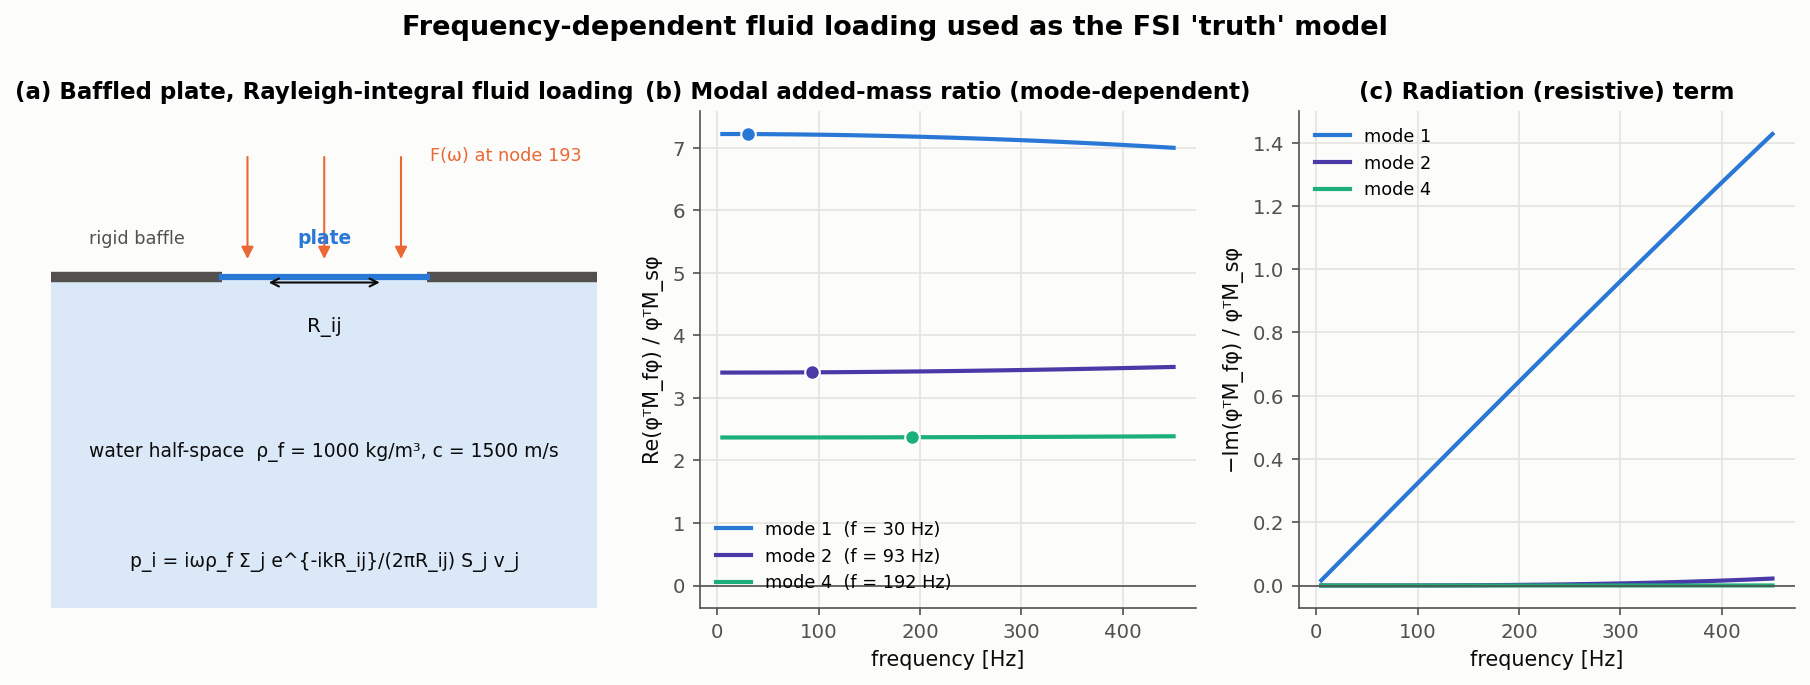
\includegraphics[width=0.9\linewidth]{figures/ch14r/fsi_fluid.png}
\caption{Frequency-dependent fluid loading. The modal added-mass ratio differs strongly by mode (about 7.2 for mode 1, 3.4 for mode 2, 2.4 for mode 4), so a uniform added mass cannot reproduce it; the radiation term grows with frequency and is largest for mode 1 (a monopole-like shape radiates efficiently).}\label{fig:vf-fsi-fluid}
\end{figure}

\begin{table}[tbp]
\centering\footnotesize
\caption{Set-up of the identification study.}\label{tab:vf-fsi-setup}
\begin{tabularx}{\linewidth}{@{}>{\raggedright\arraybackslash}p{3.2cm} >{\raggedright\arraybackslash}X@{}}
\toprule
Item & Value\\
\midrule
Plate & steel, $455\times379\times3$ mm; $E=2.1\times10^{11}$ Pa, $\nu=0.3$, $\rho_s=7850$ kg/m$^3$\\
Truth model & ANSYS finite element and boundary element model in the publication; here \texttt{Quad4MindlinPlate} 16$\times$16 and the Rayleigh-integral fluid mass\\
Sample grids, air & 17 + 17 points, 60:40:700 Hz and 80:40:720 Hz\\
Sample grids, water & 11 + 11 points, 10:40:410 Hz and 30:40:430 Hz\\
Screening & $N_{\rm ROM}=25$, $\varepsilon_f=0.5\,\%$, $\varepsilon_\eta=10\,\%$, $\tau_s=0.95$\\
Excitation / measurement cases & (1) excite 193, measure 50; (2) 193, 150; (3) 32, 58, 136, 193, 265 together, measure 50; (4) 150, 136\\
Fluid sides & one (the publication's plate is surrounded by fluid)\\
\bottomrule
\end{tabularx}
\end{table}

\Cref{fig:vf-fsi-frf} shows the only data given to the identification: the markers on the two interleaved grids against the full FRF, which the method never sees.

\begin{figure}[tbp]
\centering
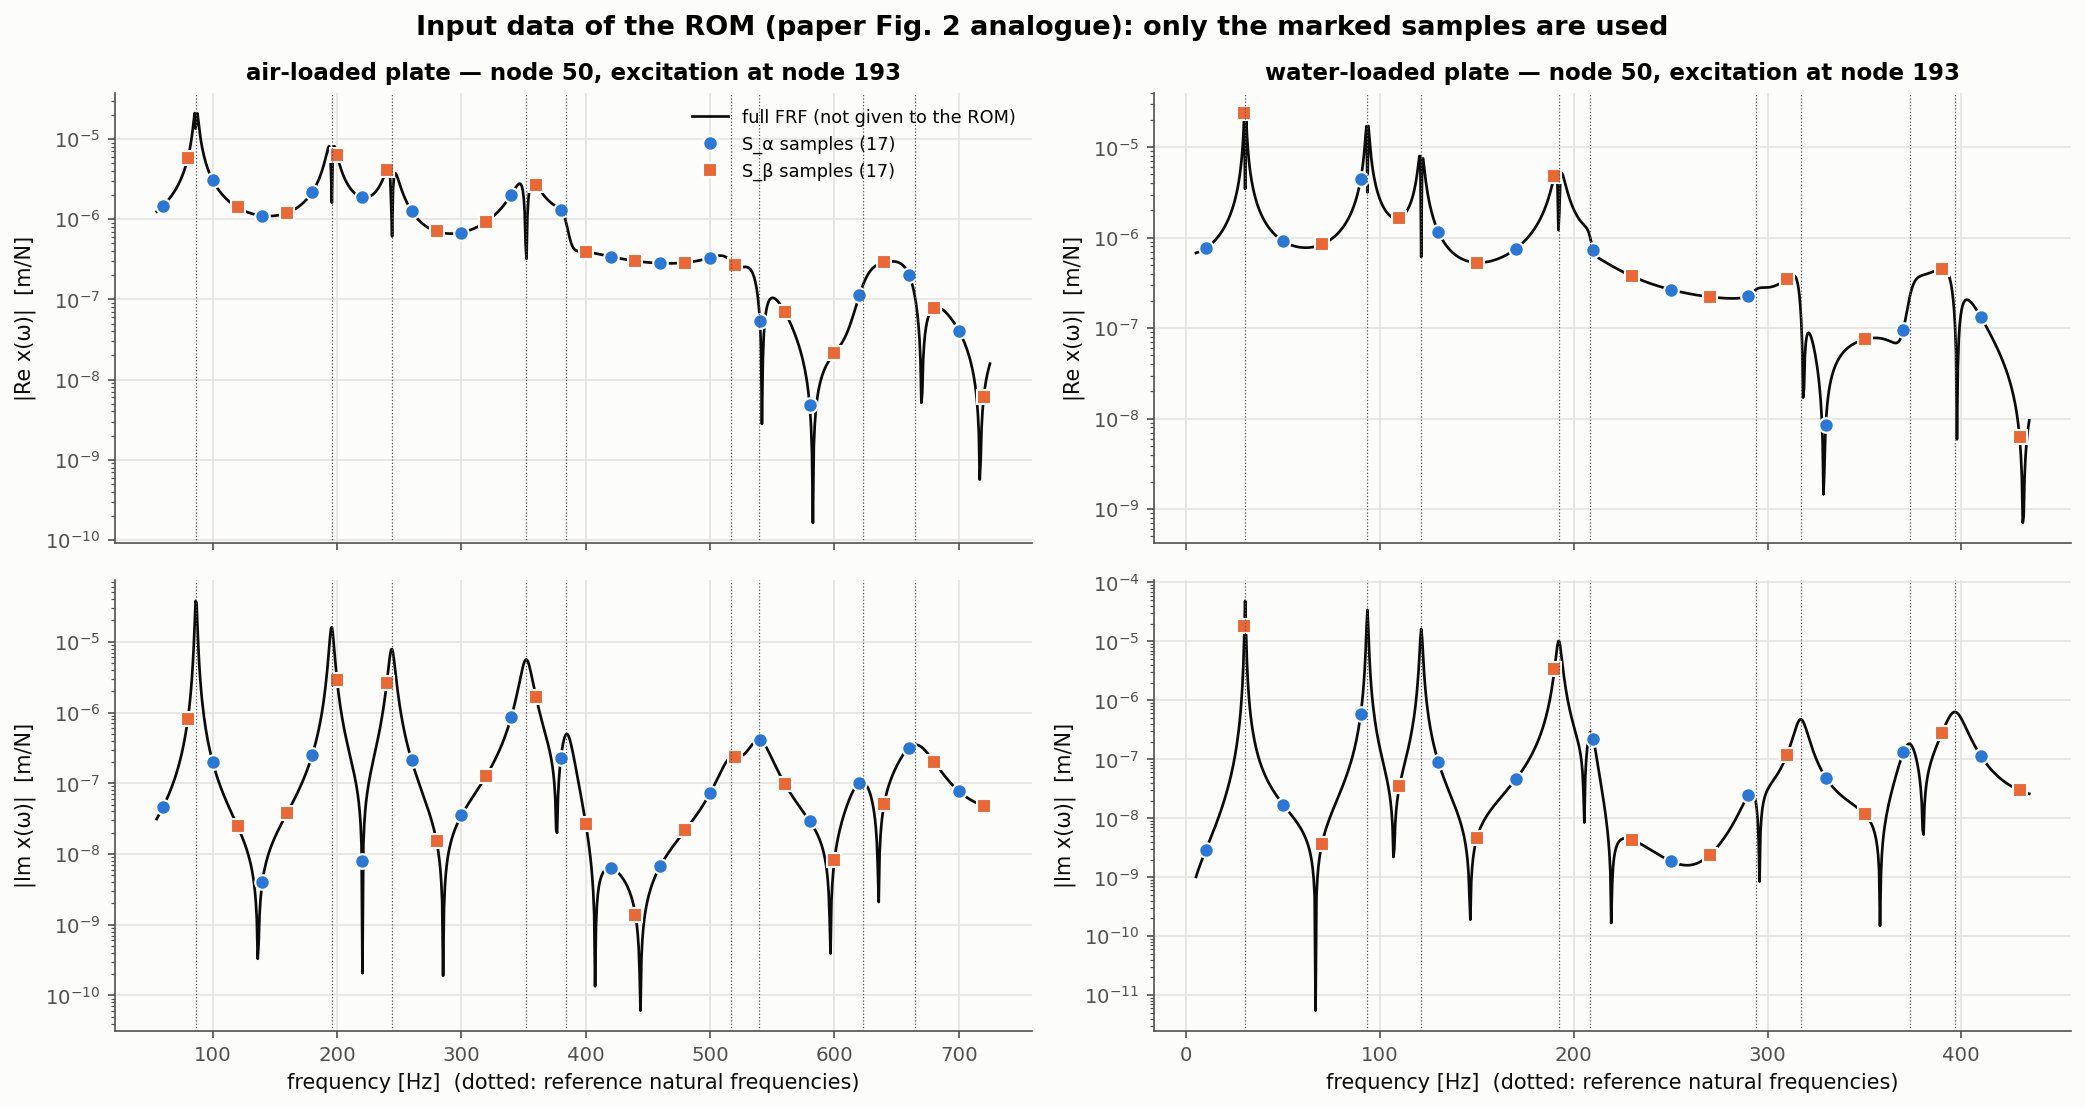
\includegraphics[width=0.9\linewidth]{figures/ch14r/fsi_frf.png}
\caption{Analogue of the publication's Fig.~2: the full FRF at node 50 for excitation at node 193 (black, not given to the method) and the samples used, on the interleaved grids (circles and squares); dotted lines are the reference natural frequencies.}\label{fig:vf-fsi-frf}
\end{figure}

\subsection*{Results: truth model against the publication (S1)}

\Cref{fig:vf-fsi-table2} compares the frequency deviation and damping ratio of the truth model with the publication's Table~2. In air the frequencies lie within $-0.3$ to $+7.2\,\%$ of the published ones ($\le1.7\,\%$ for modes 1--4) and the damping within $0.03$--$0.18$ points. In water the frequencies lie within $-9.3\,\%$ (mode 1) and $-1.1$ to $-5.0\,\%$ (modes 2--9); an earlier model with a uniform added mass was $-15$ to $-48\,\%$ off. The damping of water modes 2, 3, 4, 7, 8, 9 matches closely (mode 3: $0.570$ against $0.584$; mode 9: $1.548$ against $1.564$) but not mode 1 ($0.945$ against $0.336$), mode 5 ($1.267$ against $0.625$) or mode 6 ($1.592$ against $1.158$). The remaining differences come from model differences (Mindlin quadrilaterals against the publication's ANSYS model, a baffled half-space against its boundary-element treatment, one-sided wetting); the absolute numbers below should therefore not be compared with the publication's tables, only the behaviour of the method.

\begin{figure}[tbp]
\centering
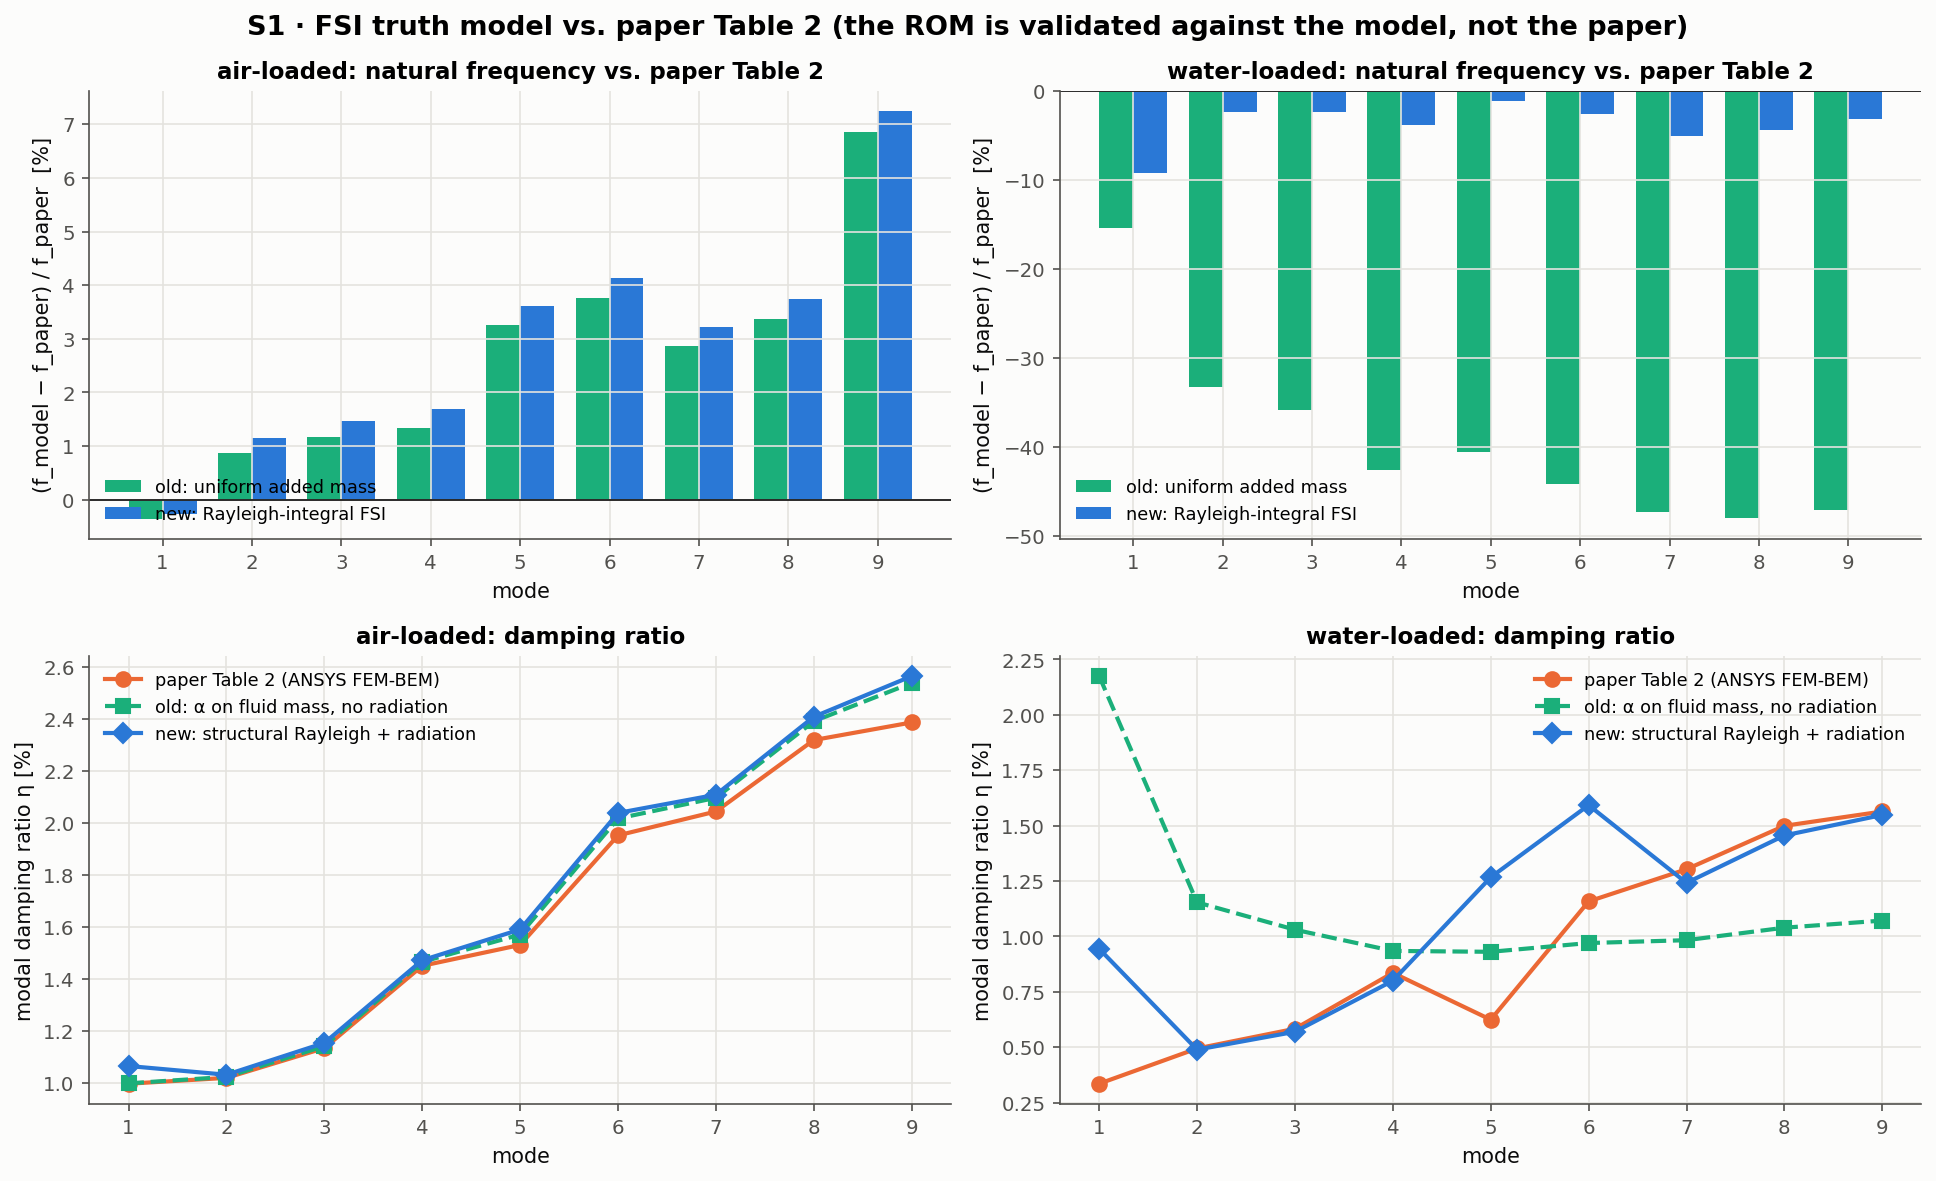
\includegraphics[width=0.9\linewidth]{figures/ch14r/fsi_table2.png}
\caption{Frequency deviation and damping ratio of the truth model against the publication's Table~2, air and water. Green: the earlier uniform-added-mass model; blue: the Rayleigh-integral model used for all studies.}\label{fig:vf-fsi-table2}
\end{figure}

\subsection*{Results: mesh, boundary condition and excitation (S2--S4)}

\emph{Mesh (S2).} \Cref{tab:vf-fsi-mesh} gives the largest ROM--FE error for three meshes in air; the publication reports below $0.2\,\%$. The method reproduces whatever mesh it is given to near round-off, because the air-loaded system is effectively frequency-independent in the band; the mode-1 frequency moves from 86.78 to 86.63 to 86.48~Hz over the meshes, which is a property of the finite element model and not of the identification.

\begin{table}[tbp]
\centering\footnotesize
\caption{Largest difference between identified and finite element frequency and damping (air).}\label{tab:vf-fsi-mesh}
\begin{tabular}{@{}lrrl@{}}
\toprule
Mesh & Frequency error & Damping error & Publication\\
\midrule
$12\times12$ & $6.7\times10^{-8}\,\%$ & $7.0\times10^{-6}\,\%$ & $<0.2\,\%$\\
$16\times16$ & $7.7\times10^{-8}\,\%$ & $6.6\times10^{-6}\,\%$ & $<0.2\,\%$\\
$24\times24$ & $4.4\times10^{-7}\,\%$ & $7.9\times10^{-6}\,\%$ & $<0.2\,\%$\\
\bottomrule
\end{tabular}
\end{table}

\begin{figure}[tbp]
\centering
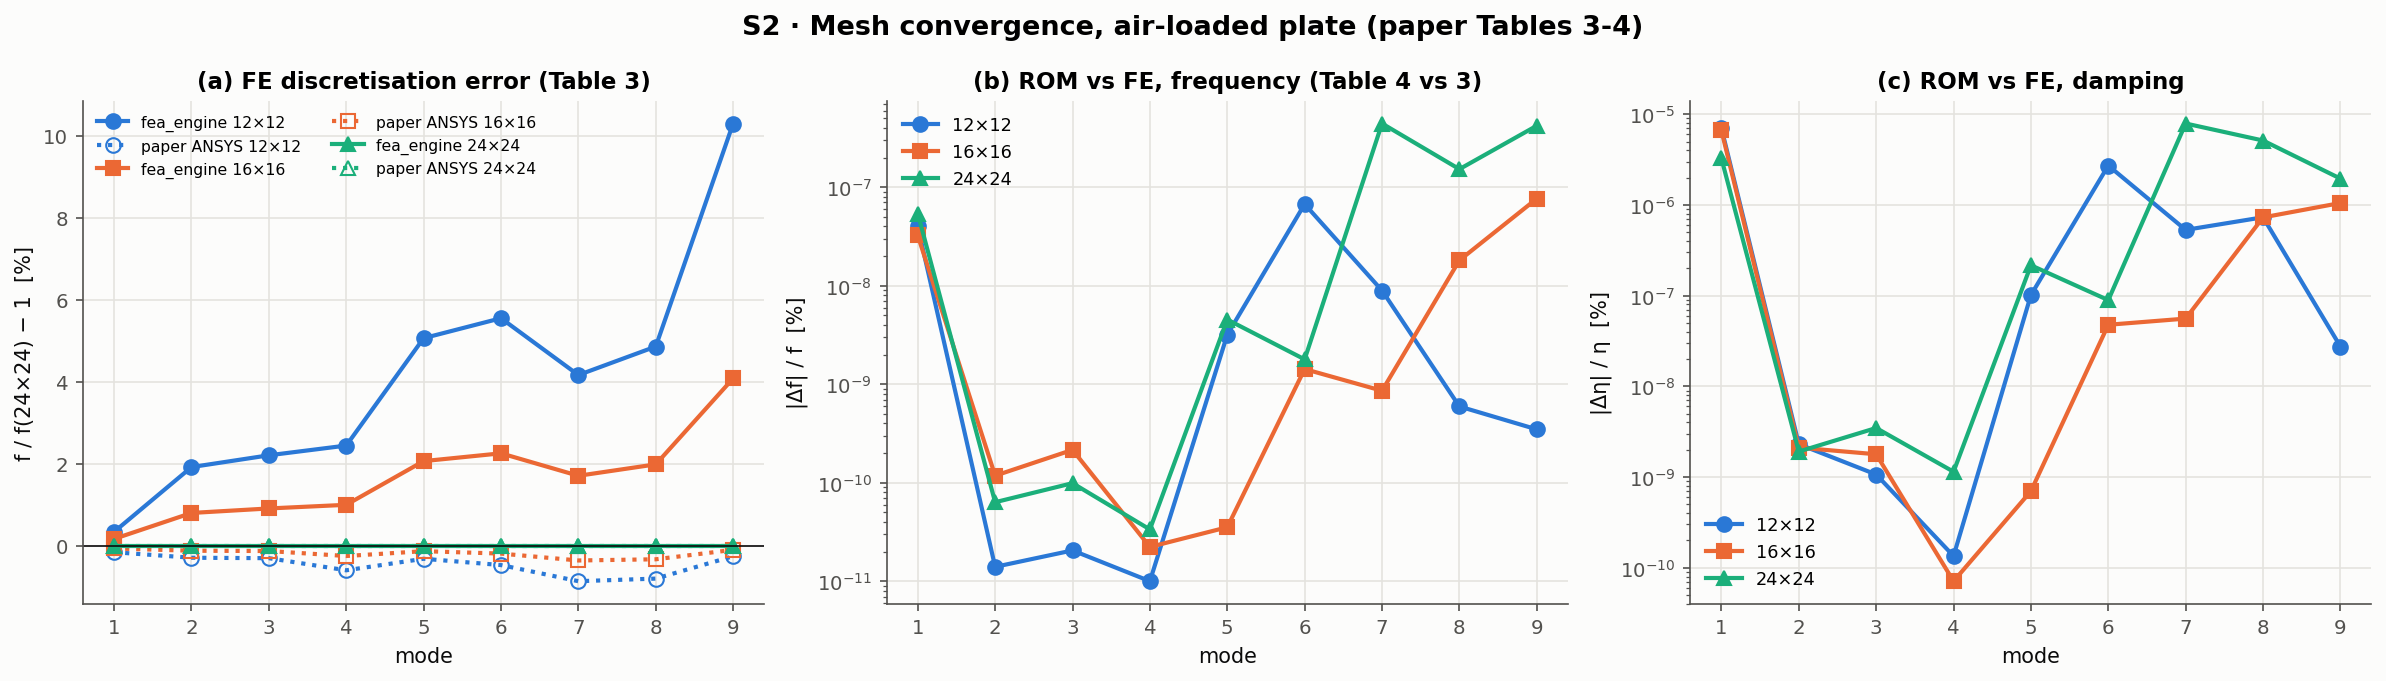
\includegraphics[width=0.9\linewidth]{figures/ch14r/fsi_mesh.png}
\caption{Reference (finite element) and identified frequency and damping for the three meshes.}\label{fig:vf-fsi-mesh}
\end{figure}

\emph{Boundary condition (S3).} For simply supported and clamped plates all nine modes are recovered with $e_f<10^{-7}\,\%$ and $e_\eta<2\times10^{-6}\,\%$; the clamped plate has mode 1 at 160.9~Hz (publication 159.5~Hz) and mode 9 at 854.7~Hz (777.5~Hz, $+9.9\,\%$). The publication's second variant with triangular shells is not covered, because the package has no triangular plate-bending element.

\emph{Excitation and measurement (S4).} \Cref{tab:vf-fsi-cases} and \Cref{fig:vf-fsi-cases} give the four configurations. Results do not depend on where the force is applied or the response measured, consistent with the publication's claim of excitation-independent identification. The $10^4$--$10^5$ times larger water error has a clear cause: the fluid mass and radiation damping of the truth model vary with frequency, so $x(\omega)$ is only approximately rational in $\omega^2$ and the pencil is no longer exact. The publication's low-error claim for water is therefore reproduced only at the $0.01$--$0.2\,\%$ (frequency) level.

\begin{table}[tbp]
\centering\footnotesize
\caption{Identification over the four excitation--measurement cases.}\label{tab:vf-fsi-cases}
\begin{tabular}{@{}lrrrrrr@{}}
\toprule
Fluid & Detected & Mean $e_f$ & Max $e_f$ & Mean $e_\eta$ & Max $e_\eta$ & Non-physical\\
\midrule
Air, all 4 cases & 9/9 & $\le7.3\times10^{-7}\,\%$ & $6.5\times10^{-6}\,\%$ & $\le2.0\times10^{-5}\,\%$ & $1.7\times10^{-4}\,\%$ & 0\\
Water, all 4 cases & 9/9 & $4.9\times10^{-3}$--$3.3\times10^{-2}\,\%$ & $0.19\,\%$ & $0.85$--$0.91\,\%$ & $4.5\,\%$ & 0\\
\bottomrule
\end{tabular}
\end{table}

\begin{figure}[tbp]
\centering
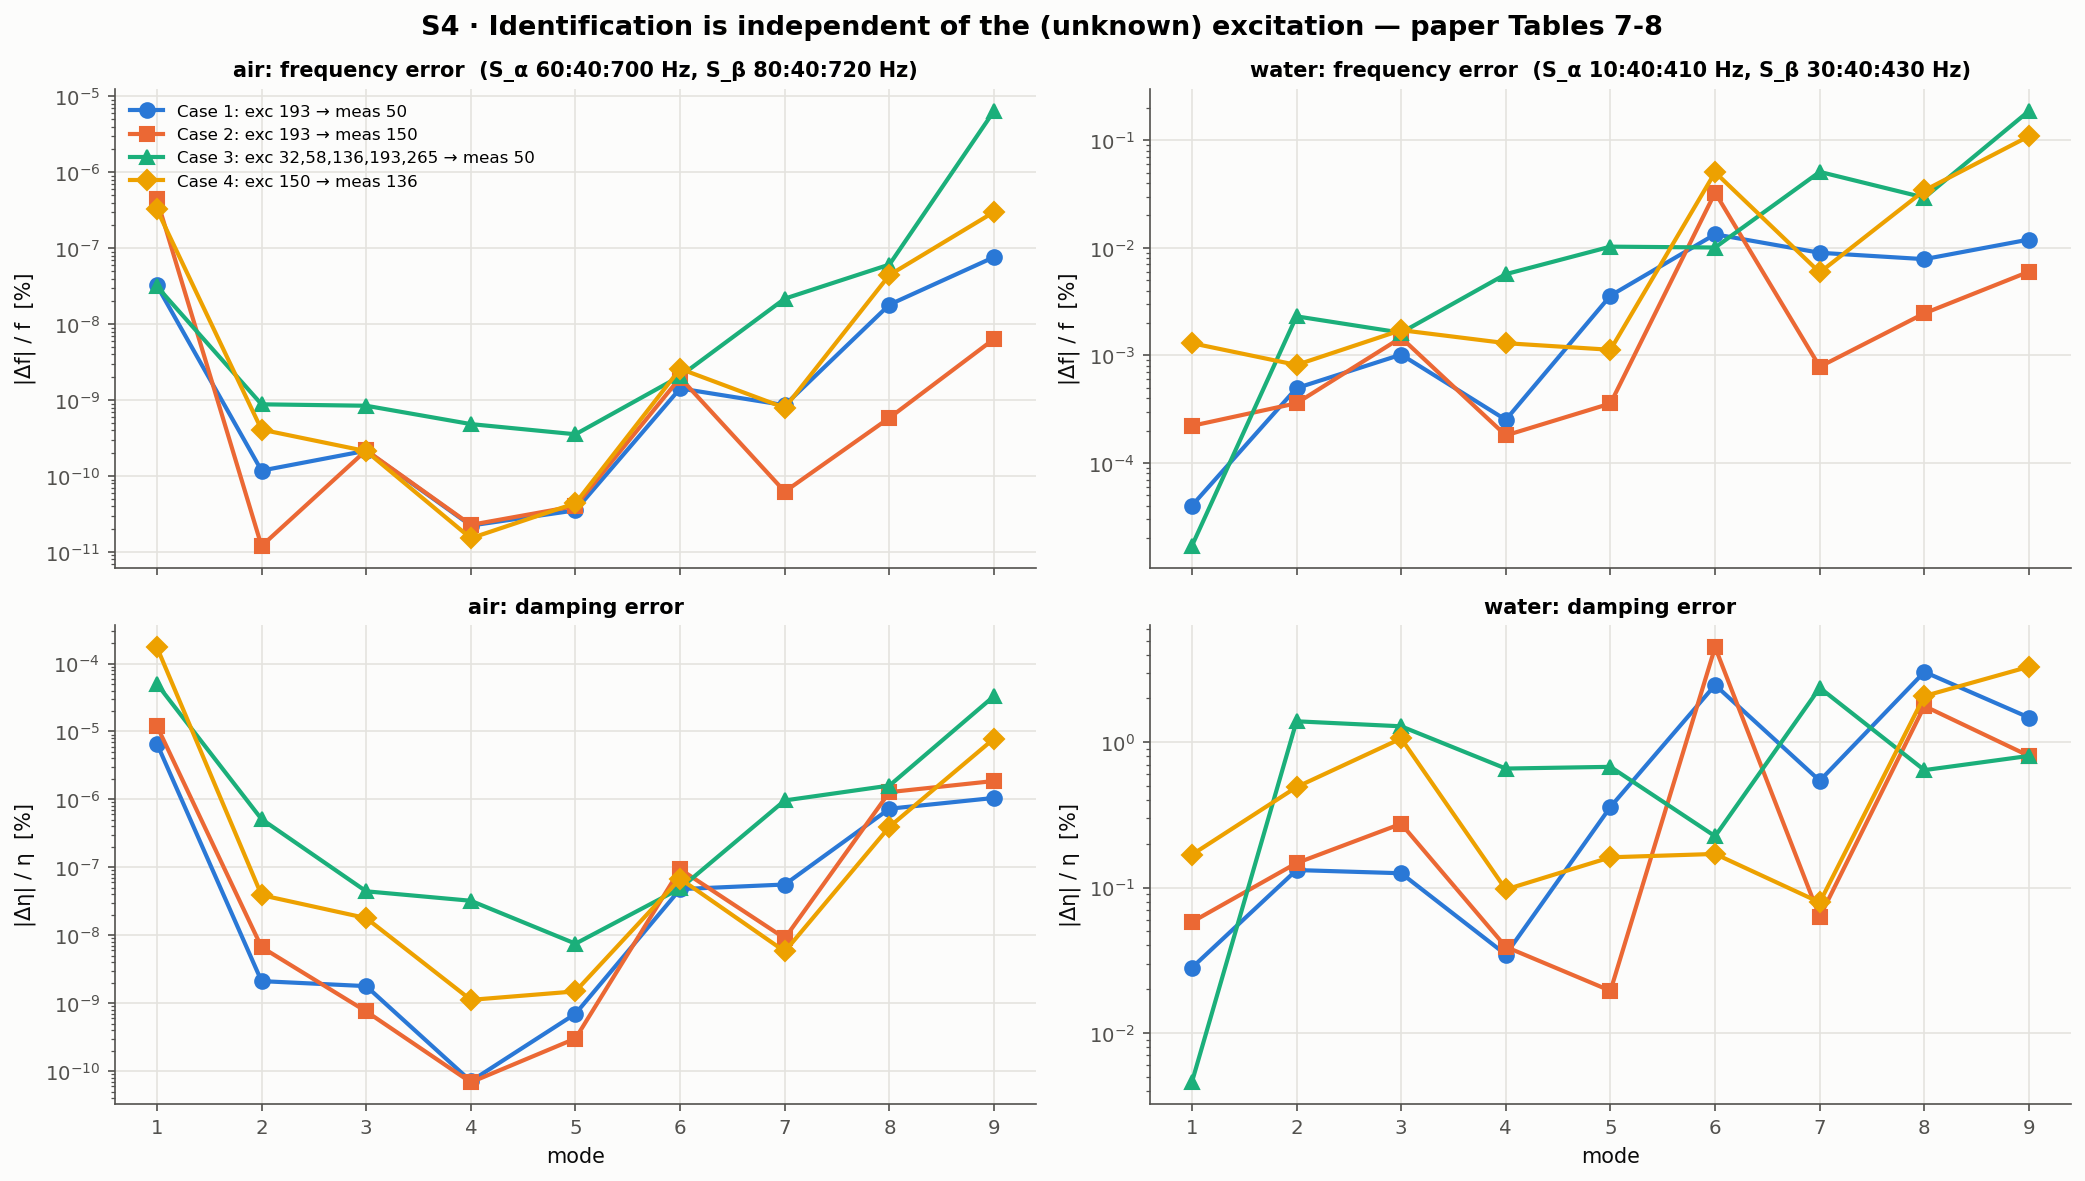
\includegraphics[width=0.98\linewidth]{figures/ch14r/fsi_cases.png}
\caption{Frequency and damping error for the four excitation--measurement configurations; left air, right water.}\label{fig:vf-fsi-cases}
\end{figure}

\subsection*{Results: sensitivity and noise (S5, S6)}

\emph{Sensitivity (water).} \Cref{fig:vf-fsi-sens} gives the mean error against (a) interpolation density, (b) frequency band, (c) sensor position and (d) excitation pattern. Errors fall monotonically as the grid is refined: mean $e_f$ is $0.36\,\%$ (18 points), $5.3\times10^{-3}\,\%$ (22), $6.0\times10^{-5}\,\%$ (26) and $1.1\times10^{-6}\,\%$ (36); with 18 points only 5 of 9 modes are detected and two spurious eigenpairs appear, and the publication's grid (22 points) gives 9 of 9 in a single model but only 5 of 9 after default screening. The wide band 0--500~Hz gives 9 of 9 even after screening, while an upper limit of 397~Hz, just below the ninth mode, loses modes (3 of 9 screened, $e_\eta\approx19\,\%$). Sensors at an edge midpoint or the plate centre detect only 6 and 3 of 9 modes, because they lie on nodal lines of the antisymmetric modes, while a corner sensor sees all nine; the modes that are seen are extremely accurate ($e_f\sim10^{-5}\,\%$). In-phase multi-point excitation leaves 1 of 9 modes after screening (single-model detection is still 9 of 9), random-phase multi-point excitation gives 6 of 9 with one spurious mode; a single point force is the most favourable pattern.

\begin{figure}[tbp]
\centering
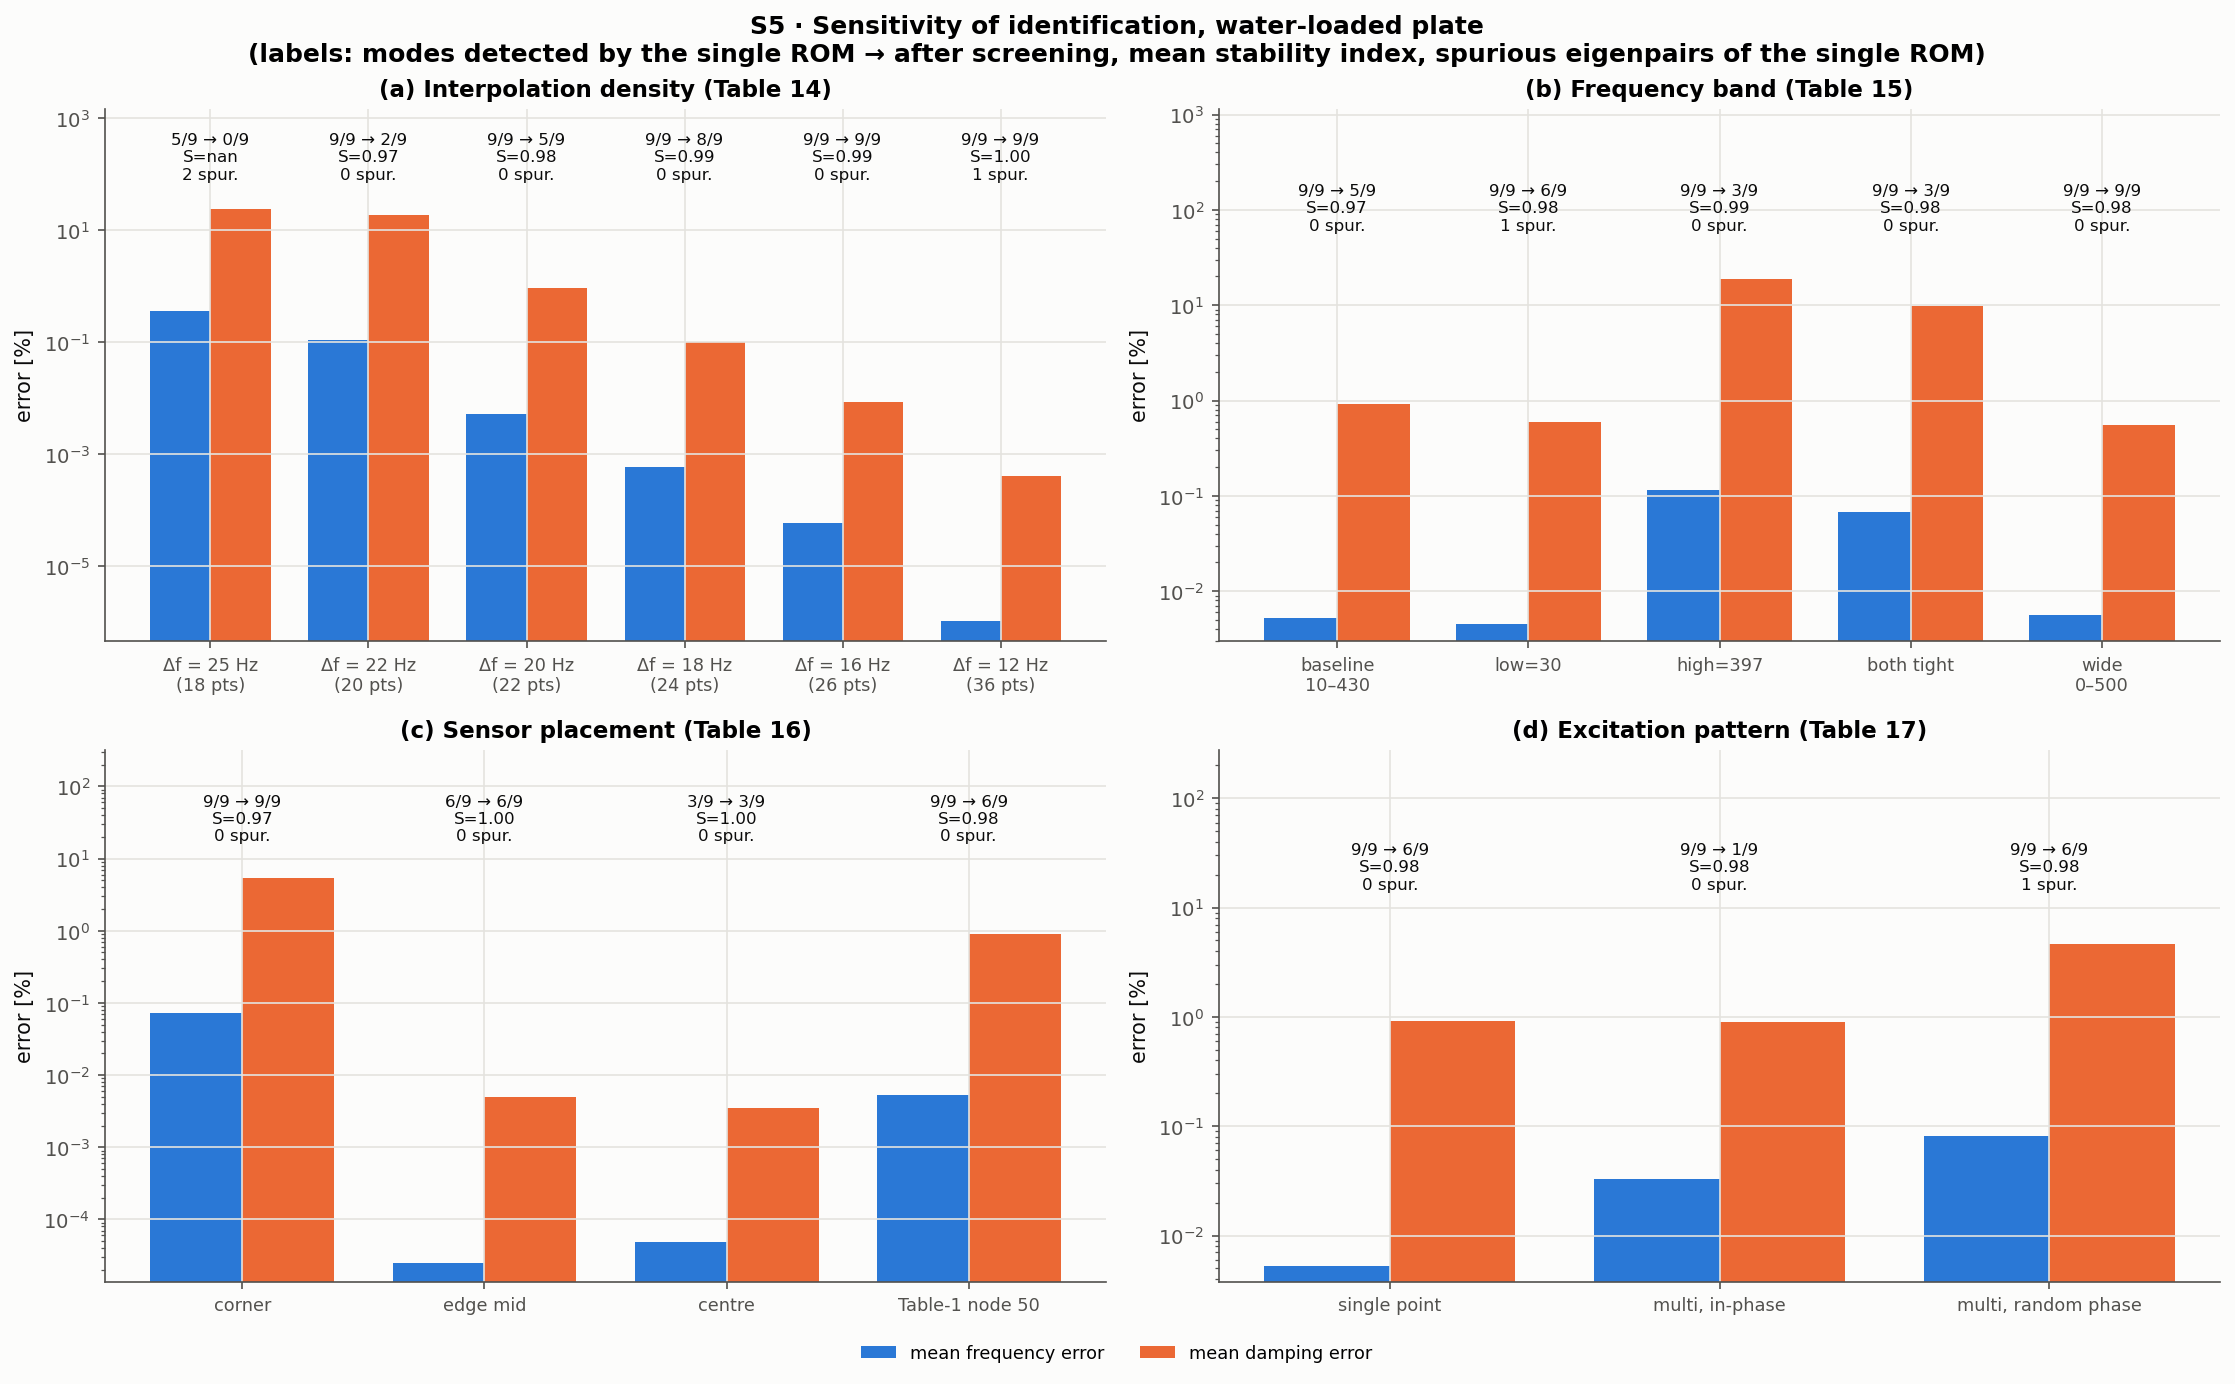
\includegraphics[width=0.98\linewidth]{figures/ch14r/fsi_sens.png}
\caption{Mean frequency (blue) and damping (orange) error against (a) interpolation density, (b) band, (c) sensor position, (d) excitation pattern, water. Labels give modes detected by a single model, after screening, the mean stability index and the number of spurious eigenpairs.}\label{fig:vf-fsi-sens}
\end{figure}

\emph{Noise.} \Cref{tab:vf-fsi-noise} and \Cref{fig:vf-fsi-noise} give median errors over 20 noise realisations per signal-to-noise ratio (SNR, 11 + 11 samples). Frequencies degrade gracefully (about $1\,\%$ even at 20~dB for the worst mode); damping is far more fragile, with errors above $10\,\%$ below about 60~dB. Screening never produced a spurious mode on the dense pool (zero at all noise levels), but at low noise ratios it also accepts almost nothing: the default thresholds ($\varepsilon_\eta=10\,\%$, $\tau_s=0.95$) were tuned on clean data, and under noise the damping scatter between models exceeds $10\,\%$, so physical modes are rejected. A noise-dependent tolerance would be needed in practice.

\begin{table}[tbp]
\centering\footnotesize
\caption{Noise robustness, water.}\label{tab:vf-fsi-noise}
\begin{tabular}{@{}rrrrrr@{}}
\toprule
SNR & Mean $e_f$ & Mean $e_\eta$ & Detected (single) & Spurious (single) & Detected (screened, 85-sample pool)\\
\midrule
20 dB & $0.90\,\%$ & $379\,\%$ & 2.7 & 3.9 & 0.0\\
40 dB & $0.67\,\%$ & $49\,\%$ & 5.3 & 2.6 & 0.3\\
60 dB & $0.27\,\%$ & $26\,\%$ & 8.0 & 1.2 & 1.8\\
80 dB & $0.06\,\%$ & $4.2\,\%$ & 9.0 & 0.2 & 6.2\\
\bottomrule
\end{tabular}
\end{table}

\begin{figure}[tbp]
\centering
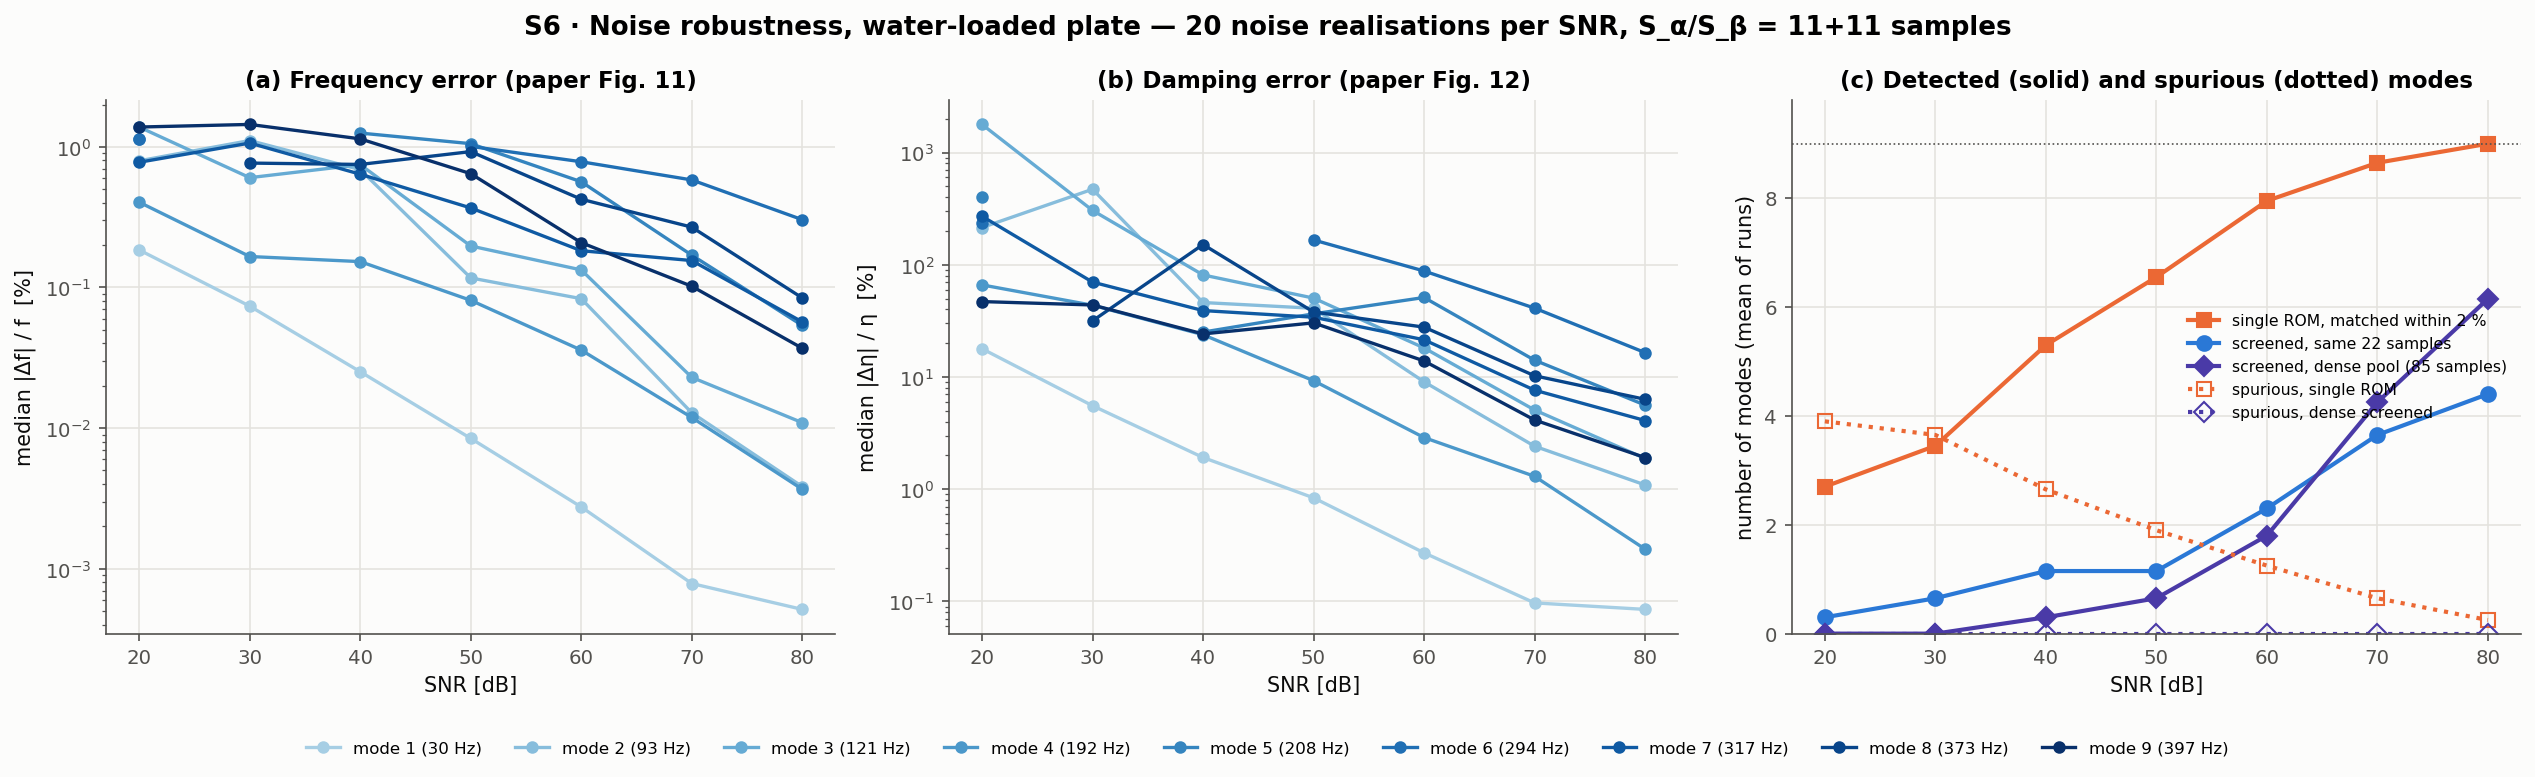
\includegraphics[width=0.98\linewidth]{figures/ch14r/fsi_noise.png}
\caption{Median error over 20 noise realisations per SNR: (a) frequency, (b) damping per mode, (c) detected (solid) and spurious (dotted) modes for a single model and for screening on 22 or 85 samples.}\label{fig:vf-fsi-noise}
\end{figure}

\subsection*{Results: mode shapes (S7)}

\Cref{tab:vf-fsi-mac} and \Cref{fig:vf-fsi-shapes,fig:vf-fsi-mac} give the shapes reconstructed as $\boldsymbol\Phi=\mathbf X_\beta\tilde\Phi$, scored by \cref{eq:fsi-mac} against the finite element shapes of the water-loaded plate. Seven of nine modes have MAC above $0.999$ on the publication-sized grid and all nine reach at least $0.9999$ on a denser $14+14$ grid; the weakest are modes 6 and 8 ($0.953$, $0.984$) and the largest off-diagonal MAC is $0.021$, so the recovered shapes are well separated. The reconstruction is real-normalised, phase-aligned and averaged over the ensemble, because the eigenvector of a single model can be badly conditioned even when its eigenvalue is accurate.

\begin{table}[tbp]
\centering\footnotesize
\caption{Mode shapes of the water-loaded plate.}\label{tab:vf-fsi-mac}
\begin{tabular}{@{}rrrrrr@{}}
\toprule
Mode & $f_{\rm ref}$ (Hz) & $f_{\rm id}$ (Hz) & MAC, 11+11 & MAC, 14+14 & Max off-diagonal\\
\midrule
1 & 30.37 & 30.37 & 1.0000 & 1.0000 & 0.017\\
2 & 93.45 & 93.45 & 0.9999 & 1.0000 & 0.006\\
3 & 121.24 & 121.24 & 0.9999 & 1.0000 & 0.001\\
4 & 192.21 & 192.21 & 1.0000 & 1.0000 & 0.000\\
5 & 208.42 & 208.41 & 0.9999 & 1.0000 & 0.017\\
6 & 293.91 & 293.95 & 0.9532 & 0.9999 & 0.021\\
7 & 317.10 & 317.07 & 0.9999 & 1.0000 & 0.001\\
8 & 373.24 & 373.21 & 0.9842 & 1.0000 & 0.004\\
9 & 396.57 & 396.52 & 0.9993 & 1.0000 & 0.006\\
\bottomrule
\end{tabular}
\end{table}

\begin{figure}[tbp]
\centering
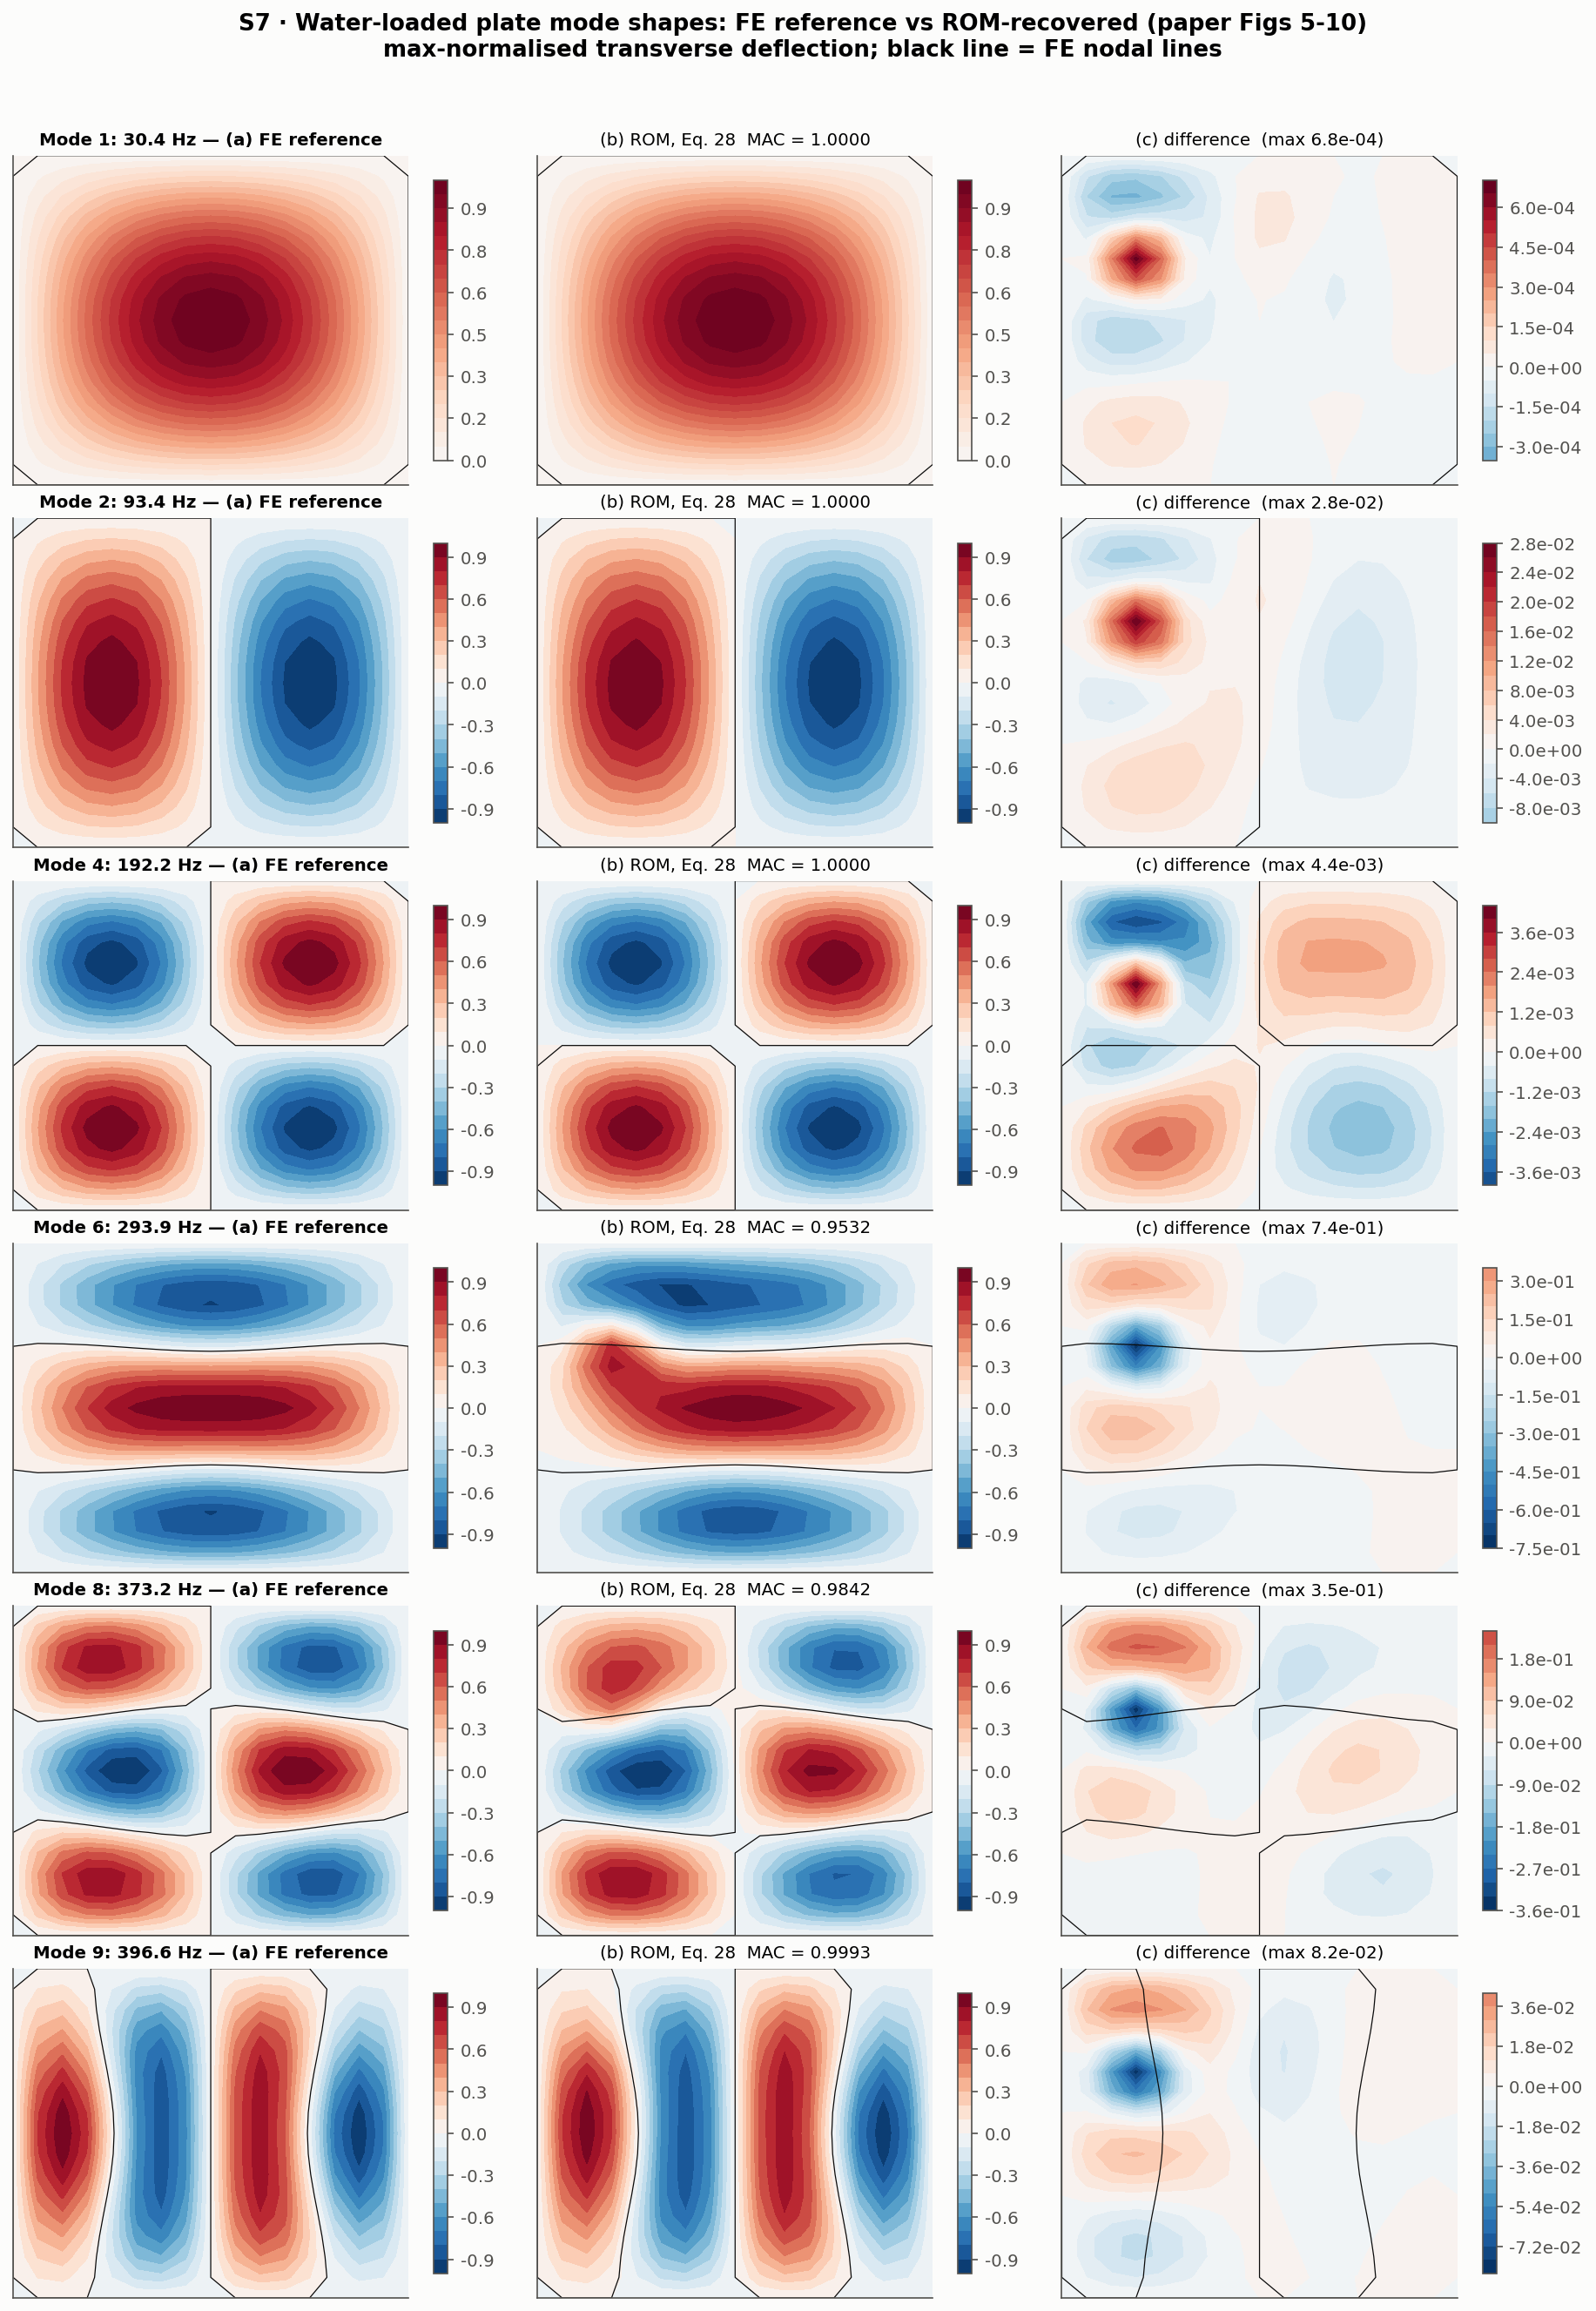
\includegraphics[width=0.98\linewidth]{figures/ch14r/fsi_shapes.png}
\caption{Identified mode shapes against finite element reference shapes, water-loaded plate.}\label{fig:vf-fsi-shapes}
\end{figure}

\begin{figure}[tbp]
\centering
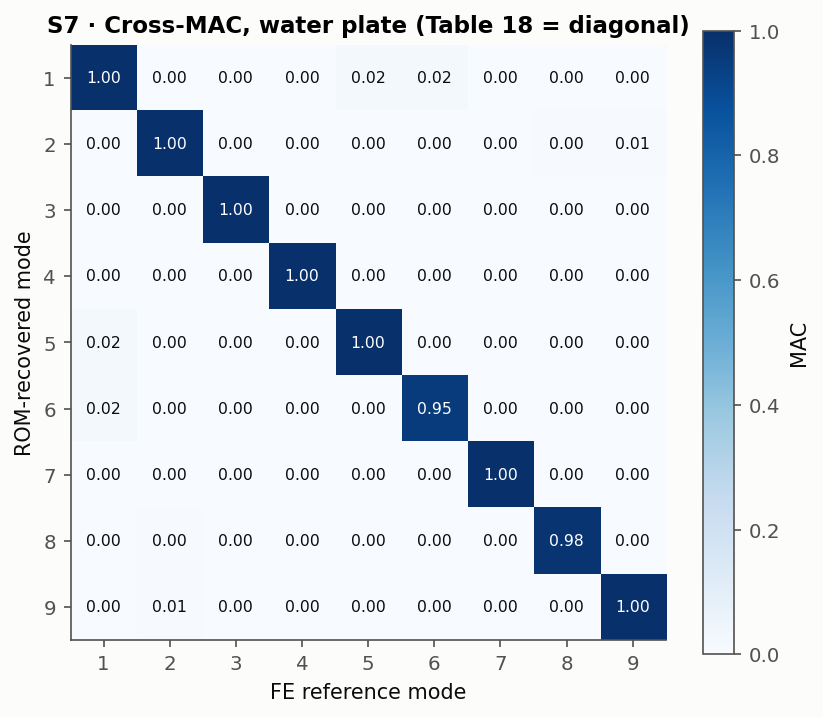
\includegraphics[width=0.6\linewidth]{figures/ch14r/fsi_mac.png}
\caption{Cross-MAC between identified and reference modes (11+11 grid); the diagonal is the publication's Table~18.}\label{fig:vf-fsi-mac}
\end{figure}

\subsection*{Comparison with the publication}

\begin{table}[tbp]
\centering\footnotesize
\caption{Claims of \citet{liu2026fsi} and the outcome against the author's own truth model.}\label{tab:vf-fsi-cmp}
\begin{tabularx}{\linewidth}{@{}>{\raggedright\arraybackslash}p{4.0cm} >{\raggedright\arraybackslash}X >{\raggedright\arraybackslash}p{2.3cm}@{}}
\toprule
Claim & This work & Outcome\\
\midrule
Frequencies and damping in air, any mesh and boundary (Tables 3--6) & errors $\lesssim10^{-5}\,\%$ & reproduced\\
Excitation- and sensor-independent identification (Tables 7--8) & 9/9 modes in all four cases; air $\le6.5\times10^{-6}\,\%$, water $\le0.19\,\%$ & reproduced\\
Water within about $0.2\,\%$ (frequency) & $0.19\,\%$ max, damping within about $5\,\%$ & reproduced at that level\\
Sensitivity to density, band, sensor, excitation (Tables 14--17) & same trends; details in figure & reproduced\\
Noise robustness (Figs.~11--12) & frequency graceful, damping fragile, screening too strict at low SNR & partly\\
Mode shapes, MAC (Table~18) & MAC $\ge0.999$ for 7 of 9, all $\ge0.9999$ on denser grid & reproduced\\
Truth model of Table~2 & air $-0.3$ to $+7.2\,\%$, water $-1.1$ to $-9.3\,\%$; damping of water modes 1, 5, 6 differs & approximate\\
\bottomrule
\end{tabularx}
\end{table}

\subsection*{Limits of the surrogate truth model}

The identification is validated against the author's surrogate truth model, not against the publication's data, because the ANSYS and boundary-element model is not available; the agreement of that model with the publication's Table~2 is only approximate (the damping of water modes 1, 5 and 6 differs). The triangular-shell model form is not covered, the fluid is one-sided where the publication's plate is surrounded by fluid, and the noise statistics use 20 realisations per level without re-tuning the screening thresholds. The report also keeps an early demonstration on a synthetic 15-degree-of-freedom mass--spring chain, which is a sanity check and not part of the results above.
